\documentclass[../main.tex]{subfiles}
\graphicspath{{\subfix{../assets/}}}

\begin{document}
\subsection{Mediu de dezvoltare și generalități}
Procesorul împreună cu celelalte circuite au fost proiectate în \acrshort{vhdl} în mediul de dezvoltare
\emph{Active-HDL Student Edition}. \emph{Active-HDL} pune la dispoziție instrumente pentru compilarea și
simularea codului \acrshort{vhdl} și Verilog. \acrshort{vhdl} este un limbaj de programare hardware. Înseamnă
că un program \acrshort{vhdl} nu poate fi rulat pe un calculator, trebuie încărcat pe o placă \acrshort{fpga},
care pe baza codului va genera circuitele și conexiunile dintre ele. E o metodă rapidă de prototipare și testare
pentru noi dispozitive hardware dar în același timp versiuni ieftine de plăci pot fi folosite în loc de
proiectarea circuitelor electronice dedicate în anumite produse.

Proiectul conține următoarele circuite ce vor fi explicate în detaliu și care pot fi observate în figura 
\ref{fig:main_block_diagram}. Pentru simplitate fiecare core al procesorului lucrează cu zone diferite
de memorie pentru a elimina necesitatea de a implementa coerența memoriei cache, deoarece un core nu va
modifica date care sunt accesibile de către celălalt core. Acest lucru a fost ușor de realizat, pentru
procesor a fost adăugat un parametru generic ce reprezintă valoarea inițială a lui \acrshort{lc}, \acrlong{lc}.
\begin{itemize}
    \item Procesor cu arhitectură \acrshort{subleq}
    \item Memorie cache cu mapare directă, \emph{write-back} cu \emph{write-allocate}
    \item Memorie RAM \emph{single port}, citire asincronă și scriere sincronă
    \item Circuit de arbitrare cu prioritate
    \item Circuit de sincronizare print \emph{handshaking}
    \item Bistabil de tip D folosit în implementarea circuitului de sincronizare (nu apare în figura \ref{fig:main_block_diagram})
\end{itemize}

\begin{figure}[h]
    \centering
    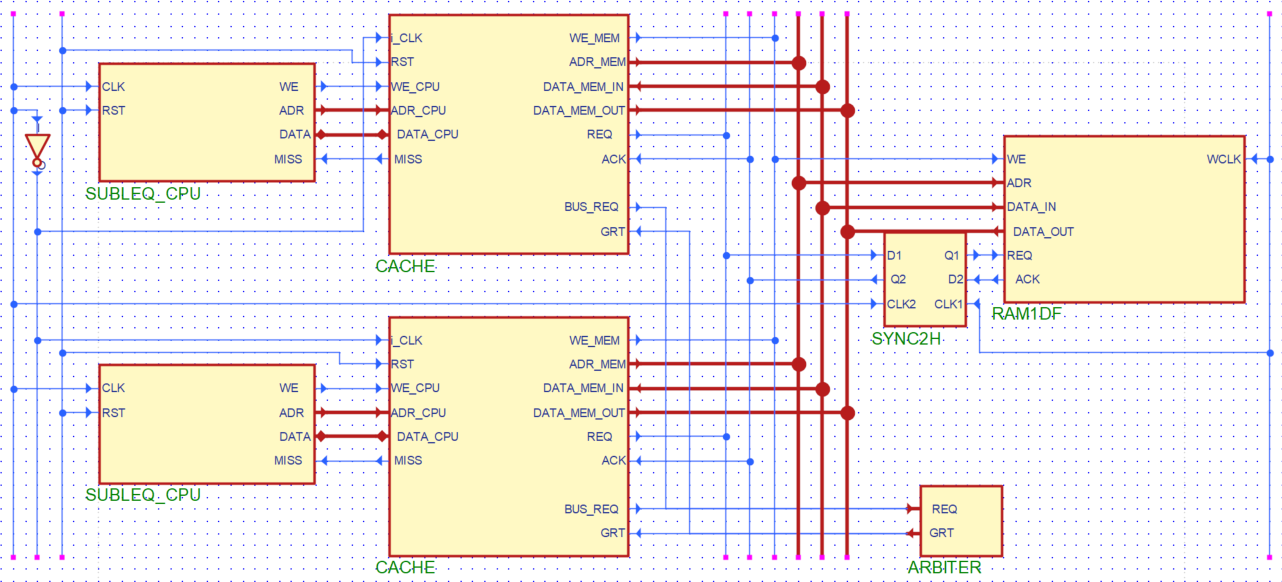
\includegraphics[width=0.9\textwidth]{main_block_diagram.png}
    \caption{Schema bloc generală}
    \label{fig:main_block_diagram}
\end{figure}

O entitate e un noțiune \acrshort{vhdl}
care descrie semnalele unui circuit. Asemenea unei interfețe care poate avea mai multe implementări, o entitate poate
avea mai multe arhitecturi. Aproape toate entitățile au și parametrii generici pentru a controla ușor numărul liniilor de date,
numărul liniilor de adresă și dimensiunea memoriilor. Fiecare semnal are un prefix în nume pentru a specifica dacă este
de intrare, de ieșire sau de intrare-ieșire.

\subsection{Implementarea procesorului SUBLEQ}
Arhitectura \acrshort{subleq} a fost aleasă din cauza popularității ei în mediul online și din cauza simplității.
Procesorul e implementat ca un automat cu stări finite care păstrează o stare internă cu informațiile necesare
pentru a putea funcționa. În figura \ref{fig:cpu_state} se pot observa stările și tranzițiile dintre acestea.
Majoritatea stărilor și desigur, majoritatea instrucțiunilor din \emph{pipeline} sunt cele de tip \emph{fetch}.
Executarea unei singure instrucțiuni \acrshort{subleq} presupune 5 operații \emph{fetch}, o operație \acrshort{alu},
o operație de scriere și încă una de decizie. Ca optimizare se verifică dacă noua valoare ce urmează să fie scrisă
este diferită de cea care există deja la acea adresă, caz în care se sare peste operația de scriere, fiind
redundantă. Optimizarea nu apare în figura \ref{fig:cpu_state}.

\begin{figure}[h]
    \centering
    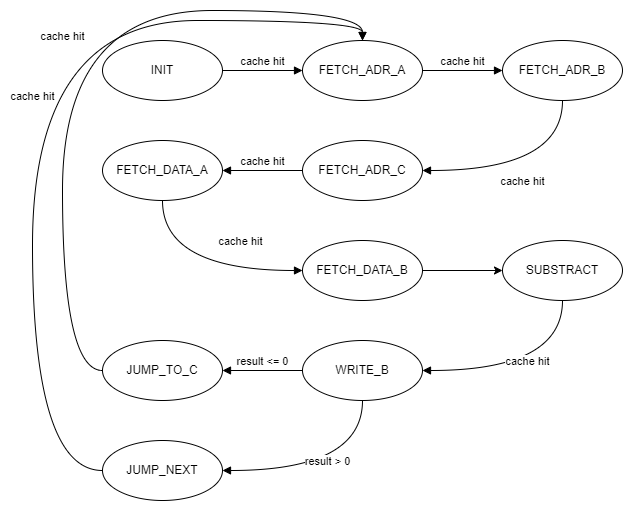
\includegraphics[width=0.8\textwidth]{cpu_state.png}
    \caption{Diagrama de stare a procesorului}
    \label{fig:cpu_state}
\end{figure}

\begin{lstlisting}[language=VHDL, caption={Entitatea procesorului}, label={lst:cpu}]
    entity SUBLEQ_CPU is
        generic(
            g_ADR_LINES  : integer := 64;
            -- bigger or equal to g_ADR_LINES due to SUBLEQ requirements
            g_DATA_LINES : integer := 64;
            g_LC_START   : integer := 0
        );
        port(
            i_CLK:   in    std_logic;
            i_RST:   in    std_logic;
            i_MISS:  in    std_logic;
            o_WE:    out   std_logic; -- WRITE ENABLE
            o_ADR:   out   std_logic_vector(g_ADR_LINES-1  downto 0);
            io_DATA: inout std_logic_vector(g_DATA_LINES-1 downto 0) 
        );
    end entity;
\end{lstlisting}

\begin{itemize}
    \item i\_CLK -- semnal de intrare -- semnalul de \emph{clock}
    \item i\_RST -- semnal de intrare -- semnal de reset, are același efect cu stare INIT din figura \ref{fig:cpu_state}
    \item i\_MISS -- semnal de intrare -- semnal de la cache, `1' în cazul unui \emph{cache miss} și `0' pentru un \emph{cache hit}
    \item o\_WE -- semnal de ieșire -- `1' pentru operația de scriere, `0' pentru citire
    \item o\_ADR -- semnal de ieșire -- adresa de la care se citește sau în care se scrie în cache
    \item io\_DATA -- semnal de intrare ieșire -- contine datele ce vor fi scrise în cache sau citite din cache de la 
    adresa specificată
\end{itemize}

\noindent\begin{minipage}{\linewidth}
Codul pseudocod pentru procesor:
\begin{lstlisting}
    LC = 0
    WHILE( TRUE )
        A = MEM[LC]
        B = MEM[LC + 1]
        C = MEM[LC + 2]
        NEW_B = MEM[B] - MEM[A]
        IF( NEW_B != MEM[B] )
            MEM[B] = NEW_B
        IF( NEW_B <= 0 )
            LC = C
        ELSE
            LC = LC + 3;
\end{lstlisting}
\end{minipage}

\subsection{Implementarea memoriei cache}
Memoria cache e cea mai importantă componentă din întregul proiect, dat fiind numărul de operații \emph{fetch} necesare
doar pentru o singură instrucțiune, plus cea de scriere. Pentru simplitate este folosită maparea directă. În acest caz
avem un număr arbitrar de linii și o linie are un număr arbitrar de blocuri de dimensiunea unui \emph{cuvânt}.
Datele dintr-o anumita adresă din memoria de nivel superior, în cazul nostru memoria RAM, pot fi stocate într-o singură
linie din cache după formula $$LINE = ADR \;\mathrm{mod}\; LINE\_COUNT$$. Din cauza asta performanța este destul de mică și numărul
de \emph{cache miss}-uri este mai mare decât în cazul celorlaltor 2 tipuri de mapări.

Din cauză că fiecare instrucțiune poate presupune o operație de scriere în memorie, strategia de scriere aleasă a fost
\emph{write-back} cu \emph{write-allocate}. Scrierea se face doar în cache, iar o linie din cache este scrisă în RAM
doar când e înlocuită ca urmare a unui \emph{cache miss}. Liniile conțin o informație suplimentară, un bit \emph{Dirty Flag}
care specifică dacă o linie trebuie sau nu să fie scrisă în memoria RAM. \emph{Dirty Flag} e setat pe 1 când are loc o
operație de scriere în cache, în felul ăsta nu se face scrierea liniei dacă nu e necesar. Figura \ref{fig:cache_state}
conține diagrama de stare a memoriei cache.

\begin{figure}[h]
    \centering
    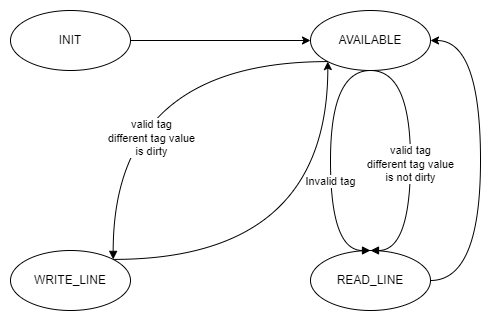
\includegraphics[width=0.7\textwidth]{cache_state.png}
    \caption{Diagrama de stare a memoriei cache}
    \label{fig:cache_state}
\end{figure}

Distingem 4 situații din figura \ref{fig:cache_state}:
\begin{itemize}
    \item Linia din care vrem să citim sau să scriem are tagul invalid, ceea ce înseamnă că încă nu a fost încarcată din memoria RAM
    nicio informație utilă, linia respectivă e goală sau contine informație inutilă. Se citește linia din memoria RAM și
    se răspunde cu \emph{cache miss}.
    \item Tagul extras din adresa de la care vrem să citim sau să scriem e diferit de tagul liniei și are \emph{Dirty Flag} setat pe 0,
    nu s-a scris în acea linie. Linia se înlocuiește și se răspunde cu \emph{cache miss}.
    \item Tagul extras din adresa de la care vrem să citim sau să scriem e diferit de tagul liniei și are \emph{Dirty Flag} setat pe 1,
    s-a scris în acea linie. Prima dată linia se este scrisă în memoria RAM și apoi se înlocuiește. Se răspunde cu \emph{cache miss}.
    \item La citire sau scriere dacă tagul liniei e valid și tagul extras din adresă e același cu tagul liniei, se execută
    operația cerută și se răspunde cu \emph{cache hit}. 
\end{itemize}

\begin{lstlisting}[language=VHDL, caption={Entitatea memoriei cache}, label={lst:cache}]
    entity CACHE is
        generic(
            g_ADR_LINES  : integer := 64;
            g_DATA_LINES : integer := 64;
            g_LINE_SIZE  : integer := 8;
            g_MEM_LINES  : integer := 32
        );
        port(
            i_CLK:      in    std_logic;
            i_ADR:      in    std_logic_vector(g_ADR_LINES-1  downto 0);
            i_DATA_MEM: in    std_logic_vector(g_DATA_LINES-1	downto 0);
            i_WE:       in    std_logic;
            i_ACK:      in    std_logic;
            i_RST:      in    std_logic;
            i_GRT:      in    std_logic;
            o_ADR:      out   std_logic_vector(g_ADR_LINES-1  downto 0); 
            o_DATA_MEM: out   std_logic_vector(g_DATA_LINES-1 downto 0);
            o_WE:       out   std_logic;
            o_MISS:     out   std_logic;
            o_REQ:      out	  std_logic;
            o_AR_REQ:   out   std_logic;
            io_DATA:    inout std_logic_vector(g_DATA_LINES-1 downto 0)
        );
    end entity;
    \end{lstlisting}

\begin{itemize}
    \item i\_CLK -- semnal de intrare -- semnalul de \emph{clock}
    \item i\_ADR -- semnal de intrare -- adresa cerută de procesor pentru a citi din cache sau scrie în cache.
    \item i\_DATA\_MEM -- semnal de intrare -- datele returnate de memoria RAM pentru adresa cerută
    \item i\_WE -- semnal de intrare -- semnal de la procesor, `1' pentru scriere, `0' pentru citire
    \item i\_ACK -- semnal de intrare -- semnal de \emph{acknewledge} de la memoria RAM pentru sincronizare 
    \item i\_RST -- semnal de intrare -- semnal de reset, are același efect cu stare INIT din figura \ref{fig:cache_state}
    \item i\_GRT -- semnal de intrare -- semnal de la arbitru, `1' înseamnă acces la \emph{bus} pentru a comunica cu memoria RAM
    \item o\_ADR -- semnal de ieșire -- adresa de la care se citește sau în care se scrie în RAM
    \item o\_DATA\_MEM -- semnal de ieșire -- semnal către RAM cu datele ce se vor scrie la adresa specificată
    \item o\_WE -- semnal de ieșire -- semnal către RAM, `1' pentru scriere, `0' pentru citire
    \item o\_MISS -- semnal de ieșire -- semnal către procesor, `1' în cazul unui \emph{cache miss}, `0' pentru \emph{cache hit}
    \item o\_REQ -- semnal de ieșire -- semnal de \emph{request} pentru scriere sincronă în RAM
    \item o\_AR\_REQ -- semnal de ieșire -- semnal către arbitru pentru a cere acces la \emph{bus}
    \item io\_DATA -- semnal de intrare ieșire -- pentru procesor, contine datele ce vor fi scrise în cache sau citite din 
    cache de la adresa specificată
\end{itemize}

\subsection{Implementarea celorlaltor circuite}
\subsubsection{Memoria RAM}
Memoria RAM servește drept spațiu de stocare principal. Datele sunt încărcate dintr-un fișier binar la începerea
simulării. Dimensiunea e specificată printr-un parametru generic. Are un singur port, ceea ce înseamnă că doar o
singură operație, de citire sau scriere, poate fi executată la un moment dat. Citirea e asincronă și de dragul
simplității presupunem că are loc destul de repede pentru a fi citită într-un singur ciclu de tact. Scrierea
e sincronă, se execută doar la semnal de \emph{clock} pe front crescător.

\begin{lstlisting}[language=VHDL, caption={Entitatea memoriei RAM}, label={lst:ram}]
    entity RAM1DF is
        generic(
            g_ADR_LINES  : integer := 64;
            g_DATA_LINES : integer := 64;
            g_MEM_SIZE   : integer := 256
        );
        port(
            i_DATA: in  std_logic_vector(g_DATA_LINES-1 downto 0);
            i_ADR:  in  std_logic_vector(g_ADR_LINES-1  downto 0);
            i_WE:   in  std_logic;
            i_WCLK: in  std_logic;
            i_REQ:  in  std_logic;
            o_DATA: out std_logic_vector(g_DATA_LINES-1 downto 0);
            o_ACK:  out std_logic := '0'
        );
    end entity;
\end{lstlisting}

\begin{itemize}
    \item i\_DATA -- semnal de intrare -- conține datele ce se vor scrie la adresa specificată
    \item i\_ADR -- semnal de intrare -- adresa din care se citește sau în care se scrie
    \item i\_WE -- semnal de intrare -- `1' pentru scriere, `0' pentru citire
    \item i\_WCLK -- semnal de intrare -- semnal de \emph{clock} pentru scrierea sincronă
    \item i\_REQ -- semnal de intrare -- semnal de \emph{request} pentru scriere
    \item o\_DATA -- semnal de ieșire -- returnează datele care se află la adresa cerută
    \item o\_ACK -- semnal de ieșire -- semnal de \emph{acknowledge} trimis după ce s-a executat scrierea, folosit pentru sincronizare
\end{itemize}

\subsubsection{Circuit de arbitrare}
Un singur core poate avea acces la \emph{bus} la un moment dat. Circuitul de arbitrare se asigură de asta. Funcționează pe
bază de prioritate, înseamnă că primul core va avea tot timpul acces la \emph{bus} în timp ce al doilea are acces doar dacă
primul core nu trimite cerere. Este implementat pentru a fi scalabil. Un parametru generic desemnează câte intrări și ieșiri
are circuitul. În \ref{fig:main_block_diagram} are 2 intrări și ieșiri pentru cele 2 core-uri.

\begin{lstlisting}[language=VHDL, caption={Entitatea arbitrului}, label={lst:arbiter}]
    entity ARBITER is
        generic(
            g_SIZE : integer := 2
        );
        port(
            i_REQ: in  std_logic_vector(g_SIZE-1 downto 0);
            o_GRT: out std_logic_vector(g_SIZE-1 downto 0)
        );
    end entity;
\end{lstlisting}

\begin{itemize}
    \item i\_REQ -- semnal de intrare -- semnale de la alte circuite pentru a cere acces la \emph{bus}
    \item o\_GRT -- semnal de ieșire -- oferă acces la \emph{bus} unui singur circuit
\end{itemize}

\subsubsection{Circuit de sincronizare}
Este folosit pentru a asigura că în timpul unei operații de scriere, semnalele implicate nu îsi schimbă valoarea până cănd
se primește un semnal de la memoria RAM cum că scrierea a fost finalizată. Cu alte cuvinte circuitul asigură sincronizarea
comunicării între 2 circuite care operează la diferite frecvențe.

\begin{lstlisting}[language=VHDL, caption={Entitatea circuitului de sincronizare}, label={lst:sync}]
    entity SYNC2H is
        port(
            i_D1:   in  std_logic;
            i_D2:   in  std_logic;
            i_CLK1: in  std_logic;
            i_CLK2: in  std_logic;
            o_Q1:   out std_logic;
            o_Q2:   out std_logic
        );
    end entity;
\end{lstlisting}

\begin{itemize}
    \item i\_D1 -- semnal de intrare -- semnal de \emph{request}
    \item i\_D2 -- semnal de intrare -- semnal de \emph{acknowledge}
    \item i\_CLK1 -- semnal de intrare -- semnal de \emph{clock} a circuitului care face \emph{request}
    \item i\_CLK2 -- semnal de intrare -- semnal de \emph{clock} a circuitului care face \emph{acknowledge}
    \item o\_Q1 -- semnal de ieșire -- semnal de \emph{request} întârziat în funcție de CLK2
    \item o\_Q2 -- semnal de ieșire -- semnal de \emph{acknowledge} întârziat în funcție de CLK1
\end{itemize}

\subsubsection{Bistabil tip D}
Circuitul de sincronizare folosește căte 2 bistabile tip D pentru fiecare semnal pentru a le întărzia cu câte 2
cicluri de tact.

\begin{lstlisting}[language=VHDL, caption={Entitatea bistabilului tip D}, label={lst:flipflopd}]
    entity D_FF is
        port(
            i_D:   in  std_logic;
            i_CLK: in  std_logic;
            o_Q:   out std_logic := '0'
        );
    end entity;
\end{lstlisting}

\begin{itemize}
    \item i\_D -- semnal de intrare -- conține datele ce vor fi salvate la următorul front crescător al semnalului de \emph{clock}
    \item i\_CLK -- semnal de intrare -- semnal de \emph{clock}
    \item o\_Q -- semnal de ieșire -- returnează datele curent salvate
\end{itemize}

\subsection{Rezultatul simulării}
Circuitul din figura \ref{fig:main_block_diagram} a fost simulat în mediul de dezvoltare \emph{Active-HDL Student Edition}
În figura \ref{fig:simple_signals} este prezentă diagrama de timp cu semnalele, în care s-a considerat un exemplu mai simplu
cu un singur core pentru a fi mai ușor de urmărit și de explicat. Printre alte considerente, dimensiunea unui cuvânt este
8 biti sau 1 octet, iar memoria cache are o singură linie cu 8 blocuri pentru a fi siguri că va avea loc o scriere în memoria
RAM. Explicația pe segmente:

\begin{figure}[h]
    \centering
    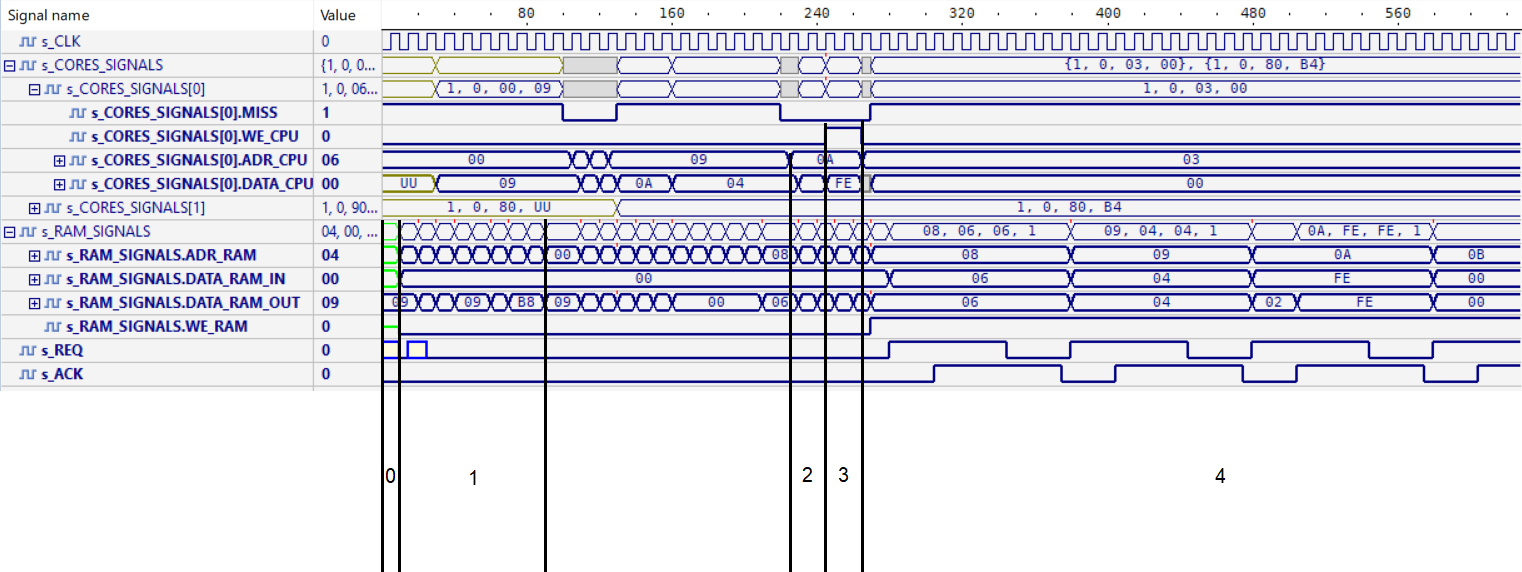
\includegraphics[width=\textwidth]{simple_signals.png}
    \caption{Diagrama de timp pe exemplu simplu}
    \label{fig:simple_signals}
\end{figure}

\begin{itemize}
    \item Segmentul 0: Conține doar partea de inițializare a circuitelor, fiecare având nevoie de un ciclu de tact.
    \item Segmentul 1: Procesorul face prima operație de citire la adresa 0x00, la acest moment singura linie din cache e
    neinițializată, adică are tagul invalid. Memoria cache trece în starea READ\_LINE și execută 8 citiri din memoria RAM,
    deoarece linia are 8 blocuri de memorie de dimendiunea unui cuvânt. În tot acest timp se trimite un semnal de
    \emph{cache miss} către procesor, iar el știe să aștepte până la un semnal \emph{cache hit} așa cum apare și în figura
    \ref{fig:cpu_state}.
    \item Segmentul 2: Aici are loc ultima operație \emph{fetch}, urmată de operația de scădere.
    \item Segmentul 3: Se execută operația de scriere prin setarea semnalului WE\_CPU pe `1'. Se scrie în aceeași
    locație de unde s-a facut ultima citire, motiv pentru care adresa rămâne aceeași.
    \item Segmentul 4: Procesorul cere datele de la adresa 0x03. Deoarece există doar o linie de cache cu 8 blocuri, asta
    înseamnă că adresa 0x03 se află în linia ce conține adresele 0x00 - 0x07. Linia curentă e 0x08 - 0xFF, știm asta pentru
    că ultima operație s-a executat pe adresa 0x0A. Se trimite un semnal \emph{cache miss} și pentru că s-a scris în
    linie trebuie să fie scrisă în RAM înainte de a fi înlocuită. Se observă 3 operații complete de scriere și una incompletă
    împreună cu semnalele de sincronizare aferente. În total o singură scriere durează 10 cicluri de tact. În cazul primelor
    2 scrieri, informația scrisă este aceiași cu cea care exista deja la adresele respective. La a 3-a scriere, în RAM este
    valoarea 0x02 și valoarea scrisă este 0xFE (-2 în complement de 2).
\end{itemize}

\end{document}